\documentclass[10pt,a4paper]{article}

\usepackage[utf8]{inputenc}
\usepackage{amsmath}
\usepackage{amsfonts}
\usepackage{amssymb}
\usepackage{fullpage}
\usepackage{svg}
\usepackage{titling}
\usepackage{tikz}
\usepackage{physics}
\usepackage{booktabs}
\usepackage{xcolor}
\usepackage{multicol}

\title{An Example of a 3D Topological Insulator: The Diamond Lattice}
\author{Alexander Heilman}

\setlength{\droptitle}{-8em}   % This is your set screw
%\setlength{\parindent}{0pt}
\begin{document}

\vspace{-3cm}
 
\maketitle

\begin{multicols}{2}

\section*{Tight-binding Hamiltonian}
Let's now consider a three dimensional system with a Hamiltonian similar to the second-order spin-orbit interaction Hamiltonian for the 2D honeycomb lattice. 
Explicitly, we now have a model for the Hamiltonian of the following form:
$$
\hat{H} = t \sum_{\langle ij\rangle ,\sigma}a^{\dagger}_{j}a_i +i\frac{8\lambda_{SOC}}{a^2}\sum_{\langle\langle ij\rangle\rangle,\sigma}c_j^{\dagger}\mathbf{s}\cdot\big( \mathbf{\hat{d}}^1_{ij}\times \mathbf{\hat{d}}^2_{ij}\big)c_i
$$
up to second nearest neighbors, where we must consider the effect of spin coupling on these second order hoppings. With $a$ the interatomic distance,
$\lambda_{SOC}$ the strength of the spin orbit coupling, and $\sigma$ denoting the spin state along some chosen axis.


We now solve for the real space expansion of this for the specific case of the diamond lattice. Much as we did before, we'll use this as a means to solve for the dispersion, by diagonalizing the $k$-space form after Fourier transforming the Fock space operators.
\section{Diamond Lattice}

For the diamond lattice, we'll assume each site has the same atom (like the colloquial diamond which is only carbon). The lattice is formed from a two point basis 
on a face centered cubic (FCC) Bravais lattice: with one atom of the basis being placed at each lattice site with displacement vector $(000)$; and the other located 
a quarter of the length along the diagonal of the cube, with the displacement vector $a\sqrt{3}/4(1,1,1)$. This lattice is depicted below, with the lighter points representing 
sublattice sites A of displacement vector 0; and the darker points representing the other sublattice, B.
\begin{center}
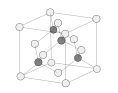
\includegraphics[scale=0.71]{diamond_uc.pdf}
\end{center}
We now need to determine the set of nearest neighbors of every site, as well as the second nearest neighbors. To accomplish this, the lattice is more easily seen in terms of the neighborhoods of both lattice sites. For the lattice sites A, we have the following neighborhoods:
\begin{center}
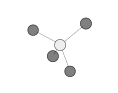
\includegraphics[scale=0.63]{diamond_a.pdf}
\end{center}
Where for each site of sublattice A, we can see there are four nearest neighbors with displacement vectors:
\begin{center}
\begin{minipage}[c]{0.6\linewidth}
\begin{itemize}
\item[$A_1$:] $a\sqrt{3}/4(1,-1,-1)$
\item[$A_2$:] $a\sqrt{3}/4(-1,1,-1)$
\item[$A_3$:] $a\sqrt{3}/4(-1,-1,1)$
\item[$A_4$:] $a\sqrt{3}/4(1,1,1)$
\end{itemize}
\end{minipage}
\end{center}
Similarly, for sublattice sites B we then have the following neighborhood 
\begin{center}
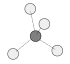
\includegraphics[scale=0.63]{diamond_b.pdf}
\end{center}
and corresponding set of displacement vectors for nearest neighbors:
\begin{center}
\begin{minipage}[c]{0.6\linewidth}
\begin{itemize}
\item[$B_1$:] $a\sqrt{3}/4(-1,1,1)$
\item[$B_2$:] $a\sqrt{3}/4(1,-1,1)$
\item[$B_3$:] $a\sqrt{3}/4(1,1,-1)$
\item[$B_4$:] $a\sqrt{3}/4(-1,-1,-1)$
\end{itemize}
\end{minipage}
\end{center}

Second nearest neighbors can be garnered from the consideration that the nearest neighbors of each sublattice are of the opposite sublattice. Hence, each second nearest neighbor has a displacement vector of the form $A_i+B_j$ with $i\neq j$ for sublattice A sites; and we then have displacement vectors of the form $B_i+A_j$ $i\neq j$ for sublattice B's second nearest neighbors. It should also now be clear that both  sites have 12 second nearest neighbors.

Now that we have the appropriate displacement vectors for the nearest and next nearest neighbors (such that we can expand the sums in an approachable manner), we consider the 
term $\mathbf{\hat{d}}^1_{ij}\times \mathbf{\hat{d}}^2_{ij}$ for each second nearest neighbor. The cross product forms a plane outlined by the two vector 'steps' taken to get to the second nearest neighbor $j$ of site $i$. The intuition is that the spins will either align or anti-align with the angular momentum of the turn at the nearest neighbor site.
\begin{center}
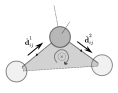
\includegraphics[scale=0.5]{diamond_nnn.pdf}
\end{center}
For completeness, we write out all of these normalized products below:
\begin{center}
\begin{minipage}[c]{0.6\linewidth}
\begin{itemize}
\item[$A_1 \ \times$] \begin{itemize}
\item[$B_2:$] $1/\sqrt{2}\ (-1,-1,0)$
\item[$B_3:$] $1/\sqrt{2}\ (1,0,1)$
\item[$B_4:$] $1/\sqrt{2}\ (0,1,-1)$
\end{itemize}
\item[$A_2\ \times$] \begin{itemize}
\item[$B_1:$] $1/\sqrt{2}(1,1,0)$
\item[$B_3:$] $1/\sqrt{2}(0,-1,-1)$
\item[$B_4:$] $1/\sqrt{2}(-1,0,1)$
\end{itemize}
\item[$A_3\  \times$] \begin{itemize}
\item[$B_1:$] $1/\sqrt{2}(-1,0,-1)$
\item[$B_2:$] $1/\sqrt{2}(0,1,1)$
\item[$B_4:$] $1/\sqrt{2}(1,-1,0)$
\end{itemize}
\item[$A_4\ \times$] \begin{itemize}
\item[$B_1:$]$1/\sqrt{2}(0,-1,1)$
\item[$B_2:$] $1/\sqrt{2}(1,0,-1)$
\item[$B_3:$]$1/\sqrt{2}(-1,1,0)$
\end{itemize}
\end{itemize}
\end{minipage}
\end{center}
Now we have all the relevant vectors for the sum expansion.

We first note that the two sublattice sites can be taken as two different orbitals with their own
respective creation and annihilation operators. We will denote these as $a^{\dagger}, a$ and $b^{\dagger}, b$ 
for the sublattice sites $A$ and $B$, respectively. 

Further, each orbital has two spin states, up and down, so that we may associate a vector of creation and annihilation operators with each orbital, namely $\vec{a}^{\dagger}, \vec{a}$ and $\vec{b}^{\dagger}, \vec{b}$. Where each of these vectors includes two components, one denoting the up spin configuration of the orbital and the other the down spin configuration of the same orbital. 

We can compose these into a $2\times 1$ vector as below:\small
\begin{align*}
\hat{H} = t \sum_{r_i }\sum_{j}\begin{bmatrix} \vec{a}_{r_i+B_j}^{\dagger} & \vec{b}_{r_i+A_j}^{\dagger} \end{bmatrix}\begin{bmatrix} 0&1\\1&0\\ \end{bmatrix}\otimes \mathbb{I}_{spin}\begin{bmatrix} \vec{a}_{r_i} \\ \vec{b}_{r_i}\end{bmatrix}\\
 +i\frac{8\lambda}{a^2}\sum_{r_i,\sigma}\sum_{j,k}\begin{bmatrix} \vec{a}_{r_i}^{\dagger} & -\vec{b}_{r_i}^{\dagger} \end{bmatrix}\mathbb{I}_{orb}\otimes\mathbf{s}\cdot\big(\hat{A}_k\times \hat{B}_j\big)\begin{bmatrix} \vec{a}_{r_i} \\ \vec{b}_{r_i}\end{bmatrix}\end{align*}\normalsize
 with the negative sign associated with $b_{r_i}$ in the second term coming from the need to switch the order of the product of $A_k$ and $B_j$ (which introduces a negative sign) for the $B\rightarrow B$, second nearest neighbor hopping. Later, this allows us to write the orbital space action as a scaled $\sigma_z$.
 
 Also, note that the left hand space of the tensor product acts on the orbital space, whereas the right hand side acts on the spin states in the any of the creation or annihilation vectors.
 
Now, recall that the spin vector takes the form $\mathbf{s}= 1/2\ (\sigma_x,\sigma_y,\sigma_z)$ for electrons, with $\sigma_i$ denoting the Pauli matrices. So, we may further expand the second nearest neighbor contribution in terms of the components of the cross product and the Pauli matrices. That is,
$$
\mathbf{s}\cdot\big(\hat{A}_k\times \hat{B}_j\big) = \sum_i c_{a_k b_j}^i\sigma_i
$$
where $c_{a_k b_j}^i$ denotes the $i$-th component of the normalized cross product $A_k\times B_j$.

Also recall that the Fourier transform of the creation and annihilation operators are of the following form:
$$
c^{\dagger}_{r_i} = \frac{1}{\sqrt{N_s}}\sum_j e^{-i\mathbf{q}\cdot\mathbf{r}_i}c_{q}^{\dagger},
$$
$$
c_{r_i} = \frac{1}{\sqrt{N_s}}\sum_q e^{i\mathbf{q}\cdot\mathbf{r}_i}c_{q};
$$
With these relations we may now expand the real space Hamiltonian, below, in terms of vectors and then transform to momentum space.\small
\begin{align*}
\hat{H} & = \sum_{r_i}\Bigg(t\sum_{j}\begin{bmatrix} \vec{a}_{r_i+B_j}^{\dagger} & \vec{b}_{r_i+A_j}^{\dagger} \end{bmatrix}\begin{bmatrix} 0&1\\1&0\\ \end{bmatrix}\otimes \mathbb{I}_{spin}\begin{bmatrix} \vec{a}_{r_i} \\ \vec{b}_{r_i}\end{bmatrix}\\
 &+i\frac{8\lambda}{a^2}\sum_{j,k}\sum_{m}\begin{bmatrix} \vec{a}_{r_i}^{\dagger} & -\vec{b}_{r_i}^{\dagger} \end{bmatrix}\mathbb{I}_{orb}\otimes c^m_{kj}\sigma_m \begin{bmatrix} \vec{a}_{r_i} \\ \vec{b}_{r_i}\end{bmatrix}\Bigg)
\end{align*}\normalsize
First, we expand the nearest neighbor sites (where we now include the spin states in the sum due to the identity in the spin space):\small
\begin{align*}
{\scriptsize \hat{H}_{\langle ij\rangle}} & = t\sum_{r_i,\sigma}\sum_{j}\begin{bmatrix} a_{r_i+B_j,\sigma}^{\dagger} & b_{r_i+A_j,\sigma}^{\dagger} \end{bmatrix}\begin{bmatrix} 0&1\\1&0\\ \end{bmatrix}\begin{bmatrix} a_{r_i,\sigma} \\ b_{r_i,\sigma}\end{bmatrix}\\
&= t\sum_{r_i,\sigma}\sum_{j} a_{r_i+B_j,\sigma}^{\dagger}b_{r_i,\sigma} + b_{r_i+A_j,\sigma}^{\dagger} a_{r_i,\sigma} \\
&= t\sum_{q,\sigma}\sum_{j} e^{-iq\cdot B_j}a_{q,\sigma}^{\dagger}b_{q,\sigma} + e^{-iq\cdot A_j} b_{q,\sigma}^{\dagger} a_{q\sigma} \\ 
&=t\sum_{q,\sigma}\sum_{j}\begin{bmatrix} a_{q,\sigma}^{\dagger} & b_{q,\sigma}^{\dagger} \end{bmatrix}\begin{bmatrix} 0&e^{-iq\cdot B_j}\\e^{-iq\cdot A_j}&0\\ \end{bmatrix}\begin{bmatrix} a_{q,\sigma} \\ b_{q,\sigma}\end{bmatrix}\\
\end{align*}\normalsize
Now, expanding the exponential in terms of the neighbors:
\begin{align*}\small
\sum_{j}e^{-iq\cdot A_j}& = e^{-i\frac{a\sqrt{3}}{4}(q_x-q_y-q_z)}+e^{-i\frac{a\sqrt{3}}{4}(-q_x+q_y-q_z)}\\
&+e^{-i\frac{a\sqrt{3}}{4}(-q_x-q_y+q_z)}+e^{-i\frac{a\sqrt{3}}{4}(q_x+q_y+q_z)}\\
\\
\sum_{j}e^{-iq\cdot B_j}& = e^{i\frac{a\sqrt{3}}{4}(q_x-q_y-q_z)}+e^{i\frac{a\sqrt{3}}{4}(-q_x+q_y-q_z)}\\
&+e^{i\frac{a\sqrt{3}}{4}(-q_x-q_y+q_z)}+e^{i\frac{a\sqrt{3}}{4}(q_x+q_y+q_z)}\\
\end{align*}\normalsize
Note that this means our operator is Hermitian (as we would hope). This can also be seen easily by considering that each displacement vector for a $A\rightarrow B$ hopping corresponds to a $B\rightarrow A$ hopping in the opposite direction. That is, $B_i=-A_i$.

Further note that we may expand the above in terms of the Pauli's (acting on the orbital subspace) by using Euler's identity for complex exponentials, that is:
$$
\begin{bmatrix}
0& e^{-i\theta}\\
e^{i\theta}& 0 \\
\end{bmatrix}= \cos\theta\ \sigma_x + \sin\theta\ \sigma_y
$$

Now we consider the second nearest neighbor term:
\tiny
\begin{align*}
\hat{H}_{\scriptsize\langle\langle ij\rangle\rangle}& = i\frac{8\lambda}{a^2}\sum_{i,j,k}\sum_{m}\begin{bmatrix} \vec{a}_{r_i}^{\dagger} & -\vec{b}_{r_i}^{\dagger} \end{bmatrix}\mathbb{I}\otimes c^m_{jk}\sigma_m \begin{bmatrix} \vec{a}_{r_i} \\ \vec{b}_{r_i}\end{bmatrix}\\
&=  i\frac{8\lambda}{a^2}\sum_{r_i,j,k}\sum_{m}\begin{bmatrix} \vec{a}_{r_i}^{\dagger} & \vec{b}_{r_i}^{\dagger} \end{bmatrix}\sigma_z\otimes c^m_{jk}\sigma_m \begin{bmatrix} \vec{a}_{q} \\ \vec{b}_{q}\end{bmatrix}\\
&=  i\frac{8\lambda}{a^2}\sum_{q,j,k}\sum_{m}\begin{bmatrix} \vec{a}_{q}^{\dagger} & \vec{b}_{q}^{\dagger} \end{bmatrix}\begin{bmatrix} e^{-iq\cdot (A_j+B_k)}&0\\0& -e^{-iq\cdot (B_j+A_k)}\\ \end{bmatrix}\\
&\hspace{5.3cm}\otimes c^m_{jk}\sigma_m \begin{bmatrix} \vec{a}_{q} \\ \vec{b}_{q}\end{bmatrix}\\
\end{align*}\normalsize
Again, expanding the exponential in terms of the neighbors, along with its corresponding Pauli vectors:
\tiny
\begin{align*}
&\sum_{j,k}^{j\neq k}\sum_{m}e^{-iq\cdot (A_j+B_k)}c_{jk}^{m}\sigma_m\\
& \ = \frac{1}{\sqrt{2}} \Big( e^{-i\frac{a\sqrt{3}}{2}(q_x-q_y)}\cdot (-\sigma_x - \sigma_y)+e^{-i\frac{a\sqrt{3}}{2}(q_x-q_z)}\cdot (\sigma_x + \sigma_z)\\
&\hspace{0.8cm} + e^{-i\frac{a\sqrt{3}}{2}(-q_y-q_z)}\cdot (\sigma_y - \sigma_z)+ e^{-i\frac{a\sqrt{3}}{2}(-q_x+q_y)}\cdot (\sigma_x + \sigma_y)\\
&\hspace{0.8cm} + e^{-i\frac{a\sqrt{3}}{2}(q_y-q_z)}\cdot (-\sigma_y - \sigma_z)+ e^{-i\frac{a\sqrt{3}}{2}(-q_x-q_z)}\cdot (-\sigma_x + \sigma_y)\\
&\hspace{0.8cm} + e^{-i\frac{a\sqrt{3}}{2}(-q_x+q_z)}\cdot (-\sigma_x - \sigma_z)+ e^{-i\frac{a\sqrt{3}}{2}(-q_y+q_z)}\cdot (\sigma_y+ \sigma_z)\\
&\hspace{0.8cm} + e^{-i\frac{a\sqrt{3}}{2}(-q_x-q_y)}\cdot (\sigma_x - \sigma_y)+ e^{-i\frac{a\sqrt{3}}{2}(q_y+q_z)}\cdot (-\sigma_y + \sigma_z)\\
&\hspace{0.8cm} + e^{-i\frac{a\sqrt{3}}{2}(q_x+q_z)}\cdot (\sigma_x - \sigma_z)+ e^{-i\frac{a\sqrt{3}}{2}(q_x+q_y)}\cdot (-\sigma_x + \sigma_y)\Big)\\
& \ = \sqrt{2} \Big[\sin\Big(\frac{a\sqrt{3}}{2}(q_x-q_y)\Big) \cdot (\sigma_x + \sigma_y)+\sin\Big(\frac{a\sqrt{3}}{2}(-q_x+q_z)\Big) \cdot (\sigma_x + \sigma_z)\\
&\hspace{0.8cm} +\sin\Big(\frac{a\sqrt{3}}{2}(q_y+q_z)\Big) \cdot (\sigma_y - \sigma_z)+\sin\Big(\frac{a\sqrt{3}}{2}(q_y-q_z)\Big) \cdot (\sigma_y + \sigma_z)\\
&\hspace{0.8cm} +\sin\Big(\frac{a\sqrt{3}}{2}(-q_x-q_z)\Big) \cdot (\sigma_x - \sigma_z)+\sin\Big(\frac{a\sqrt{3}}{2}(q_x+q_y)\Big) \cdot (\sigma_x - \sigma_y)\Big]\\
\end{align*}\normalsize
And, applying the triginotmetric identity $\sin(x+y)=\sin(x)\cos(y)+\cos(x)\sin(y)$, we may simplify the above and collect terms as follows:\footnotesize
\begin{align*}
&\ = 2\sqrt{2}\Big[ \sin\big( \frac{a\sqrt{3}}{2} q_x\big) \Big( \cos\big( \frac{a\sqrt{3}}{2} q_y\big) -\cos\big( \frac{a\sqrt{3}}{2} q_z\big) \Big) \sigma_x \\
&\hspace{0.83cm} +\sin\big( \frac{a\sqrt{3}}{2} q_y\big) \Big( \cos\big( \frac{a\sqrt{3}}{2} q_z\big) -\cos\big( \frac{a\sqrt{3}}{2} q_x\big) \Big) \sigma_y\\
&\hspace{0.83cm} +\sin\big( \frac{a\sqrt{3}}{2} q_z\big) \Big( \cos\big( \frac{a\sqrt{3}}{2} q_x\big) -\cos\big( \frac{a\sqrt{3}}{2} q_y\big) \Big) \sigma_y\ \Big]\\
\end{align*}\normalsize
We now have all of the components of the momentum space Hamiltonian, and expand the terms we've collected in the basis of the tensor product of two Paulis, acting on the orbital space (left hand) and the spin space (right hand). The basis $\Gamma^{i}$ is defined as the following:
$$
\begin{array}{c  c  c  c  c}
\Gamma^1&\Gamma^2&\Gamma^3&\Gamma^4&\Gamma^5\\
\sigma^x\otimes \mathbb{I} &\sigma^y\otimes \mathbb{I} 
&\sigma^z\otimes \sigma^x &\sigma^z\otimes \sigma^y
 &\sigma^z\otimes \sigma^z \\
\end{array}
$$
And in which we seek a form of the  Hamiltonian:
$$
\hat{H}=d_0(\mathbf{k})\mathbb{I} + \sum_{a=1}^5 d_a(\mathbf{k})\Gamma^i
$$
Now, collecting the coefficients of these terms from our previous considerations, we have the following:
\footnotesize
$$
\begin{array}{l c}
d_0(\mathbf{k}):& 0\\
d_1(\mathbf{k}):& t\sum_{i}\cos(\mathbf{q}\cdot A_i) \\
d_2(\mathbf{k}):& t\sum_{i}\sin(\mathbf{q}\cdot A_i)\\
d_3(\mathbf{k}):& i\frac{16\sqrt{2}\lambda}{a^2}\sin\big( \frac{a\sqrt{3}}{2} q_x\big) \Big( \cos\big( \frac{a\sqrt{3}}{2} q_y\big) -\cos\big( \frac{a\sqrt{3}}{2} q_z\big) \Big)  \\
d_4(\mathbf{k}):&  i\frac{16\sqrt{2}\lambda}{a^2}\sin\big( \frac{a\sqrt{3}}{2} q_y\big) \Big( \cos\big( \frac{a\sqrt{3}}{2} q_z\big) -\cos\big( \frac{a\sqrt{3}}{2} q_x\big) \Big)\\
d_5(\mathbf{k}):& i\frac{16\sqrt{2}\lambda}{a^2}\sin\big( \frac{a\sqrt{3}}{2} q_z\big) \Big( \cos\big( \frac{a\sqrt{3}}{2} q_x\big) -\cos\big( \frac{a\sqrt{3}}{2} q_y\big) \Big)\\
\end{array}
$$\normalsize
From which we may easily get the band structure in degenerate pairs:
$$
E(\mathbf{k}) = d_0(\mathbf{k})\pm \sqrt{ \sum_{a=1}^5 d_a(\mathbf{k})^2}
$$

\subsection{Topological Invariants}
We now consider a modulation along each nearest neighbor bond (such that we may relax the symmetry of the lattice and introduce some anisotropy) of the form:
$$
t\rightarrow t_i= t+\delta t_i
$$
where each nearest neighbor bond $A_i$ now has a (potentially) unique hopping parameter $t_i$.

We can then solve for the value of the topological invariants $\delta_i$ from our previous form for the Hamiltonian according to
\begin{align*}
\delta_{n_1n_2n_3} & = -\text{sgn}\big[d_1(\vec{q}=\Gamma_{n_1n_2n_3})\big]\\
& = -\text{sgn}\big[\sum_{i}t_i\cos(\Gamma_{n_1n_2n_3}\cdot A_i)\big]\\
\end{align*}
where $\Gamma_i$ are the time-reversal invariant momentum (TRIM) and which take the values
$$
\Gamma_{n_1n_2n_3}=\frac{1}{2}\big(n_1\vec{b}_1+n_2\vec{b}_2+n_3\vec{b}_3\big)
$$
with $n_i=0,1$, and $\vec{b}_i$ being the FCC reciprocal lattice vectors, which are here defined as the following in terms of components:
\begin{align*}
\vec{b}_1 & = \frac{2\pi}{a}(-1,1,1)\\
\vec{b}_2 & = \frac{2\pi}{a}(1,-1,1)\\
\vec{b}_3 & = \frac{2\pi}{a}(1,1,-1)\\
\end{align*}
Since the underlying lattice of the diamond structure is face-centered cubic, this reciprocal lattice is body-centered cubic (as is clear from the reciprocal lattice vectors).
\begin{center}
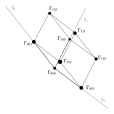
\includegraphics[scale=0.5]{diamond_gamma.pdf}
\end{center}
Now, noting that $\Gamma \cdot A_k = n_k\pi$, we can easily determine the invariant of every gamma point (here with only $\delta t_3 \neq 0$, and assumed to be small relative to $t$):
\begin{align*}
\underline{ (i,j,k)}\ &\ \underline{ \delta_{(i,j,k)}}\\
(0,0,0)& \ \ \ -1\\(0,0,1)& \ \ \ -1\\
(0,1,0)& \ \ \ -1\\
(0,1,1)& \ \ \ \text{sgn}[\delta t_3]\\(1,0,0)& \ \ \ -1\\
(1,0,1)& \ \ \ \text{sgn}[\delta t_3]\\(1,1,0)& \ \ \ -\text{sgn}[\delta t_3]\\
(1,1,1)& \ \ \ +1\\
\end{align*}
The topological invariant of the bulk is then the product of all of these invariants, which is simply $\text{sgn}[\delta t_3]$. Thus, the bulk material is a strong topological insulator (characterized by an invariant of value $-1$) for negative $\delta t_3$, and a weak topological insulator for positive $\delta t_3$. 

Two dimensional surfaces or faces of the diamond lattice then may be specified by (perpendicular) reciprocal lattice vectors $G_{(\nu_1\nu_2\nu_3)}$ of the form below:
$$
G_{\nu_1\nu_2\nu_3}=\nu_1\vec{b}_1+\nu_2\vec{b}_2+\nu_3\vec{b}_3
$$
Each surface also has it's own topological properties, which may be described according to a set of topological invariants. These invariants may be characterized (much like the bulk or a two-dimensional material) by the coefficient of $d_1$ at certain surface TRIM. These surface TRIM are specified as $\Lambda_{a}$ which are projections of bulk TRIM $\Gamma_{ai}$ onto the surface under consideration (specified by some $G$) and where the $\Gamma_{ai}$ pairs satisfy:
$$
\Gamma_{a1}-\Gamma_{a2}=G_a/2
$$
\end{multicols}

\begin{thebibliography}{2}
\bibitem{diamond} Liang Fu, C. L. Kane, and E. J. Mele, Topological insulators in three dimensions, PHYS REV LETT 98, 106803 (2007)

\bibitem{topins} Liang Fu and C. L. Kane, Topological insulators with inversion symmetry, PHYSICAL REVIEW B 76, 045302 (2007)
\end{thebibliography}
\end{document}